
\subsubsection{Cycle enumeration}
\subparagraph{Current implementation}
The only available implementation is for directed graphs. It works by first
getting SCCs
(\href{https://en.wikipedia.org/wiki/Strongly_connected_component}{strongly
    connected components}) and then deleting the
\href{https://en.wikipedia.org/wiki/Bridge_(graph_theory)}{bridges} (any edge
between two different SCCs) from the graph (similar to Johnson’s
algorithm\cite{johnson1975}). This prunes a lot of paths that might be
traversed later but will never result in a cycle (no cycle ever contains a
bridge). It then starts by calling a BFS
(\href{https://en.wikipedia.org/wiki/Breadth-first_search}{breadth-first
    search}) from all starting vertices. The BFS ensures that all the cycles
starting at the same vertex are yielded in increasing order of length. For
multiple cycles starting at different vertices, we store the shortest cycle
from each vertex in a heap. When a cycle needs to be returned, the shortest
cycle is extracted from the heap and yielded, and then the next shortest cycle
starting from the same vertex is added to the heap again.

\begin{algorithm}[H]
    \caption{$simple\ cycles\ in\ a\ directed\ graph$}
    \begin{algorithmic}[1]
        \Require A digraph $D = (V,A)$, a set of startix vertices $S \subseteq V$
        \Ensure Simple cycles in $D$ yielded by increasing length
        \Function{$\_all\_cycles\_iterator\_vertex$}{$v$}
        \State $queue \gets [[v]]$
        \While{$queue$ not empty}
        \State Extract $p$ from $queue$
        \If{$p$ is a simple cycle}
        \State \textbf{yield} $p$
        \Else
        \For{every neighbor $v' \in V$ of last vertex of $p$}
        \State $p' \gets p + v'$
        \If{$p'$ is simple path or simple cycle}
        \State append $p'$ to the end of $queue$
        \EndIf
        \EndFor
        \EndIf
        \EndWhile
        \EndFunction

        \Function{$all\_cycles\_iterator$}{$S$}
        \State $SCCs \gets$ strongly connected components of $D$
        \State $brideges \gets []$
        \For{each $v \in V$}
        \For{each edge $e = vv', v' \in V, e \in A$}
        \If{$v$ and $v'$ are in different $SCCs$}
        \State add $e$ to $brideges$
        \EndIf
        \EndFor
        \EndFor
        \State $A \gets A \setminus brideges$
        \State $heap \gets$ an empty heap
        \For{$v \in S$}
        \State add iterator \Call{$\_all\_cycles\_iterator\_vertex$}{$v$} to $heap$
        \EndFor
        \While{$heap$ not empty}
        \State Extract $iterator$ from $heap$, containing current shortest cycle
        \State $shortest\_cycle \gets$ from $iterator$
        \State $iterator \gets$ next element from $iterator$
        \If{$iterator$ not empty}
        \State append $iterator$ to $heap$
        \EndIf
        \State \textbf{yield} $shortest\_cycle$
        \EndWhile
        \EndFunction
    \end{algorithmic}
\end{algorithm}

\subparagraph{Proposed approaches}
\begin{itemize}
    \item \textbf{For undirected graphs}: SCC doesn’t apply directly.
          We could run the above algorithm without dividing the graph first,
          but this would lead to many unnecessary computations,
          as the BFS would start visiting paths that never yield a cycle.
          Instead, I propose using \textbf{BCCs} (\href{https://en.wikipedia.org/wiki/Biconnected_component}{biconnected components}).
          Biconnected components divide the graph into multiple components
          such that starting the BFS from vertices
          within a component—without traversing between components—ensures
          no extra paths (which cannot form cycles) are explored.
          \begin{figure}[htbp]
              \centering
              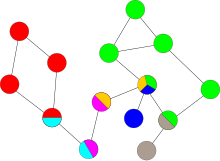
\includegraphics[width=0.8\textwidth]{Project/Details/Graph-Biconnected-Components.png} % Adjust width/height
              \caption{An example for Biconnected components in a graph}
              \label{fig:example}
          \end{figure}
          \begin{algorithm}[H]
              \caption{$simple\ cycles\ in\ a\ undirected\ graph$ (modified from algorithm 1)}
              \begin{algorithmic}
                  \State at line 1
                  \State \textbf{function} $\_all\_cycles\_iterator\_vertex(v, BCCs)$
                  \State \ldots
                  \State starting from line 8
                  \For{every neighbor $v' \in V$ of last vertex of $p$, such that $v'$ belong to the same biconnected component as $p$ in $BCCs$}
                  \State $p' \gets p + v'$
                  \If{$p'$ is simple path or simple cycle}
                  \State append $p'$ to the end of $queue$
                  \EndIf
                  \EndFor
                  \State \ldots
                  \State replaces lines 18 to 27
                  \State $BCCs \gets$ biconnected components of $D$
                  \State \ldots
                  \State at line 29
                  \For{$v \in S$}
                  \State add iterator \Call{$\_all\_cycles\_iterator\_vertex$}{$v, BCCs$} to $heap$
                  \EndFor
                  \State \ldots
              \end{algorithmic}
          \end{algorithm}
          This ensures that the shortest simple cycles are yielded without any drawbacks to efficiency compared to the method for directed graphs.

    \item \textbf{For weighted graphs}:
          the BFS finds shortest cycles first by searching by breadth,
          but for weighted graphs it cannot adapt
          to that since it never considers the weight and only considers
          the edges themselves. What I propose is adapting to a \href{https://en.wikipedia.org/wiki/Dijkstra's_algorithm}{Dijkstra}-like method,
          that is, by using a heap instead of a queue and storing
          and sorting based on the current path weight in the heap.
          This will ensure that the cycles with the smallest weight are retrieved first.
          \begin{algorithm}[H]
              \caption{$simple\ cycles\ in\ a\ weighted\ graph$ (modified from both algorithms 1 \& 2)}
              \begin{algorithmic}
                  \State \ldots
                  \State in $\_all\_cycles\_iterator\_vertex$
                  \State $heap \gets [(0,[v])]$ \Comment{a heap storing a path and its weight, while sorting on the weight}
                  \While{$heap$ not empty}
                  \State Extract $(w,p)$ from $heap$
                  \If{$p$ is a simple cycle}
                  \State \textbf{yield} $(w,p)$
                  \Else
                  \For{every neighbor $v' \in V$ of last vertex of $p$}
                  \State $p' \gets p + v'$
                  \State $w' \gets w + w(vv')$ \Comment{new weight of $p'$}
                  \If{$p'$ is simple path or simple cycle}
                  \State append $(w',p')$ to the $heap$
                  \EndIf
                  \EndFor
                  \EndIf
                  \EndWhile
                  \State \ldots
              \end{algorithmic}
          \end{algorithm}
\end{itemize}

\subparagraph{Deliverables}
These are the tasks that are expected to be delivered for this part of the
project.

\begin{itemize}
    \item Simple cycles in undirected graph
    \item Extend methods to support weighted graphs
\end{itemize}

Each and every task will contain the following

\begin{itemize}
    \item Core implementation
    \item Testing
    \item Documentation
\end{itemize}

All methods will follow a consistent input/output format:
\begin{itemize}
    \item \textbf{Input}: Parameters specifying cycle properties (e.g., length bounds, weight thresholds).
    \item \textbf{Output}: Iterators yielding cycles in ascending order of weight/length.
\end{itemize}


